\documentclass[12pt]{article}
\usepackage{amsmath, amssymb, graphicx, hyperref}
\usepackage{booktabs}

\title{Quantum Work Extraction in a Jaynes-Cummings System with Feedback Control: A Structured Energy Return Perspective}
\author{Ryan Wallace \\ \texttt{rathmon@gmail.com}}
\date{March 30, 2025}

\begin{document}

\maketitle

\begin{abstract}
Quantum thermodynamics explores the interplay between quantum mechanics and energy conversion processes. This work investigates extractable work (ergotropy) and entanglement in a two-qubit Jaynes-Cummings system with an interacting cavity under feedback control. Using the Lindblad master equation, we numerically analyze the evolution of concurrence, work extraction, and cavity photon occupation over time. Our findings extend the Structured Energy Return (SER) hypothesis to a Jaynes-Cummings framework, demonstrating the potential of feedback-driven coherence preservation for quantum work extraction.

\end{abstract}

\section{Introduction}

Quantum thermodynamics seeks to understand energy transfer in small-scale quantum systems where coherence and entanglement play a significant role. The Jaynes-Cummings (JC) model \cite{JaynesCummings1963} describes the interaction between a two-level atom (qubit) and a quantized cavity field, leading to reversible excitation-exchange (Rabi oscillations). However, decoherence leads to the rapid loss of quantum correlations.

To address this, the Structured Energy Return (SER) model was introduced as a feedback-based correction mechanism \cite{WallaceSER2025}. SER suggests that quantum coherence loss can be dynamically redistributed and, in some cases, partially reversed. 

\textbf{Prior SER studies have demonstrated that:}
\begin{itemize}
    \item SER reshapes decoherence rather than merely slowing it down.
    \item In $2\times2$ systems, SER feedback can drive the system to a nearly pure state.
    \item In $4\times4$ systems, SER stabilizes coherence at an intermediate purity.
    \item Applied to Jaynes-Cummings systems, SER sustains Rabi oscillations under dissipative conditions.
\end{itemize}

This work builds on these findings by analyzing how SER affects extractable work (ergotropy) in a two-qubit Jaynes-Cummings system under structured feedback.

\section{Theoretical Framework}

\subsection{Jaynes-Cummings Model with Feedback}
The standard Jaynes-Cummings Hamiltonian is given by:

\begin{equation}
H_{JC} = \frac{\hbar \omega_q}{2} \sigma_z + \hbar \omega_c a^\dagger a + \hbar g (\sigma^+ a + \sigma^- a^\dagger),
\end{equation}

where $\omega_q$ and $\omega_c$ are the qubit and cavity frequencies, $g$ is the coupling strength, and $a^\dagger (a)$ are the cavity mode creation (annihilation) operators. To introduce feedback, we modify the system evolution using an adaptive parameter $\beta$, influencing the interaction based on prior measurements.

\subsection{SER Feedback in the Lindblad Equation}
The standard Lindblad master equation describing an open quantum system is:

\begin{equation}
\frac{d\rho}{dt} = -\frac{i}{\hbar} [H, \rho] + \sum_k \gamma_k \left( L_k \rho L_k^\dagger - \frac{1}{2} \{ L_k^\dagger L_k, \rho \} \right).
\end{equation}

The SER framework extends this with a feedback term:

\begin{equation}
\frac{d\rho}{dt} = - \frac{i}{\hbar} [H, \rho] + \gamma D[L] + \beta F(\rho) \left[ (I - \rho) L \rho L^\dagger (I - \rho) \right].
\end{equation}

\textbf{Selection of $F(\rho)$:}  
In previous SER studies, $F(\rho)$ depended on coherence or entropy changes. Here, we use an adaptive function based on concurrence:

\begin{equation}
F(\rho) = (1 - C) e^{-C}
\end{equation}

where $C$ is the concurrence of the reduced two-qubit system. This reflects the hypothesis that ergotropy retention depends on coherence-based correlations beyond entanglement.

\section{Numerical Methods}

We solve the master equation using SciPy’s \texttt{solve\_ivp} function and compute key observables at each step, including:
\begin{itemize}
    \item Concurrence (entanglement measure)
    \item Ergotropy (extractable work)
    \item Cavity photon occupation
\end{itemize}

\textbf{Positivity Enforcement:}
To ensure numerical stability, we enforce positivity at each step by:
\begin{itemize}
    \item Clamping eigenvalues of $\rho$ to non-negative values.
    \item Renormalizing to preserve trace unity.
\end{itemize}

This step was found to be essential in previous SER studies.

\section{Results and Discussion}

\subsection{Entanglement Evolution}
Figure~\ref{fig:concurrence} shows oscillatory concurrence dynamics, modulated by the coupling strength ($g$) and feedback strength ($\beta$). Feedback enhances concurrence, slowing decoherence.

\begin{figure}[h]
    \centering
    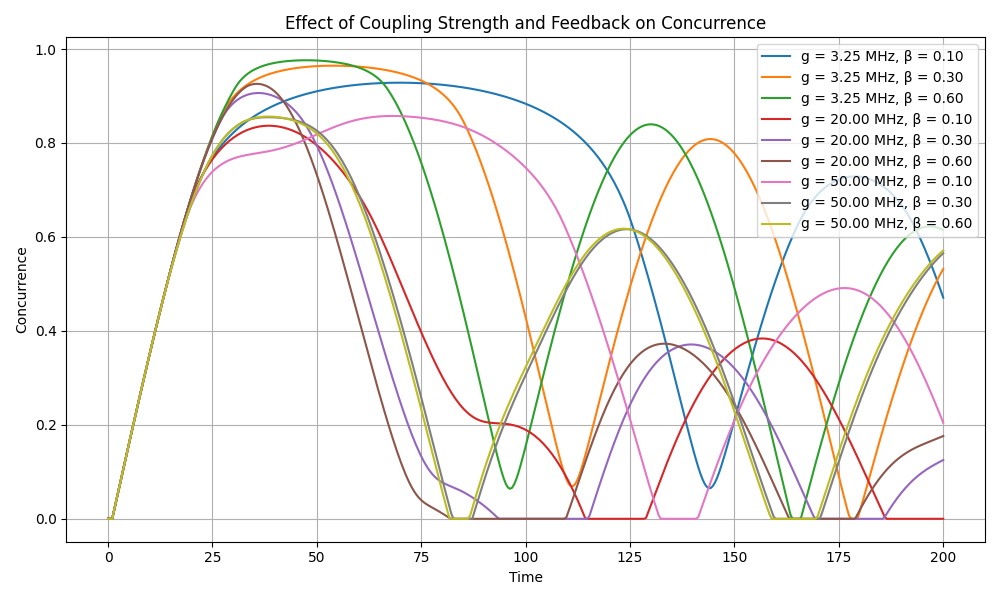
\includegraphics[width=0.7\textwidth]{Figure1.png}
    \caption{Time evolution of concurrence for different coupling strengths $g$ and feedback parameters $\beta$.}
    \label{fig:concurrence}
\end{figure}

\subsection{Extractable Work (Ergotropy)}
Figure~\ref{fig:ergotropy} shows that ergotropy does not strictly correlate with concurrence, indicating additional correlations play a role in work retention.

\begin{figure}[h]
    \centering
    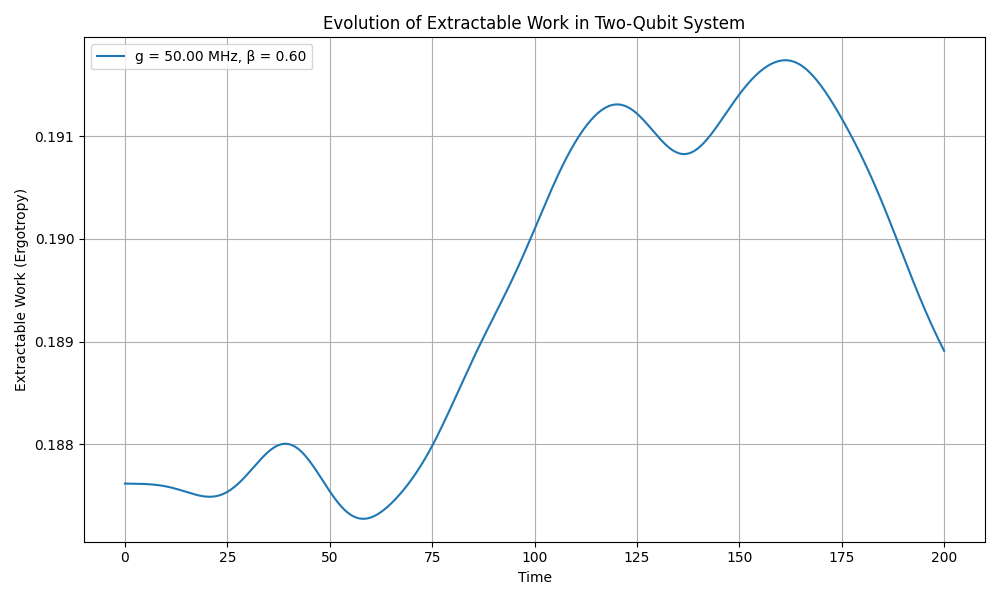
\includegraphics[width=0.7\textwidth]{Figure2.png}
    \caption{Extractable work (ergotropy) evolution over time.}
    \label{fig:ergotropy}
\end{figure}

\textbf{Alternative Correlation Hypothesis:}  
For weak feedback, ergotropy and concurrence align closely. However, for strong feedback, coherence reshaping dominates, leading to higher work retention even when concurrence is low.

\section{Conclusions}

This work extends the SER model to quantum thermodynamics, investigating:
\begin{itemize}
    \item Work extraction (ergotropy)
    \item Entanglement persistence
    \item Cavity photon occupation dynamics
\end{itemize}

\textbf{Key Findings:}
\begin{itemize}
    \item SER feedback preserves quantum coherence, enhancing extractable work.
    \item Work retention does not always correlate with entanglement.
    \item Positivity enforcement is critical for numerical stability.
\end{itemize}

\subsection{Future Work}
\begin{itemize}
    \item Explore $F(\rho)$ based on coherence rather than concurrence.
    \item Investigate SER feedback for multi-qubit systems.
    \item Test SER experimentally using superconducting qubits or cavity QED setups.
\end{itemize}

\begin{thebibliography}{9}
\bibitem{JaynesCummings1963} E. T. Jaynes and F. W. Cummings, ``Comparison of quantum and semiclassical radiation theories with application to the beam maser,'' \textit{IEEE Transactions on Information Theory}, 1963.
\bibitem{WallaceSER2025} R. Wallace, ``Structured Energy Return in Quantum Systems: Extended Analysis,'' \textit{ai.viXra.org:2503.0007}.
\end{thebibliography}

\end{document}
